\chapter[Metodologia]{Metodologia}\label{ch:metodologia}

Este capítulo tem o objetivo de apresentar a metodologia da monografia bem como os processos que serão seguidos a fim de atingir os objetivos da pesquisa. O capítulo está divido em duas seções: a Seção x apresenta ..., e a Seção Y apresenta 

%\section{Considerações iniciais}
(a terminar)


Será adotada a metodologia Scrum - descrita na Seção \ref{sec:scrum} - para apoiar a metodologia de desenvolvimento de software (Seção \ref{sec:metodologia_desenvolvimento}).

\section{Metodologias de pesquisa}

O conhecimento científico diverge dos demais tipos de conhecimento devido à necessidade de adotar fundamentação e metodologias a serem seguidas. Além disso, baseia-se em \textit{“informações classificadas, submetidas à verificação, que oferecem explicações plausíveis a respeito do objeto ou evento em questão”} \cite[pág. 22]{prodanov2013}. Ou seja, é imprescindível determinar o método científico que possibilitou atingir esse conhecimento \cite[pág. 24]{prodanov2013}. 

A pesquisa científica, por sua vez, tem por finalidade descobrir respostas para questões mediante a aplicação de um \textit{“(...) processo formal e sistemático de desenvolvimento do método científico. O objetivo fundamental da pesquisa é descobrir respostas para problemas mediante o emprego de procedimentos científicos.”}  \cite[pág. 26]{gil2008}.

Quanto aos objetivos, é possível classificar as pesquisas em três categorias \cite[pág. 41]{gil2002}: (i) exploratória, (ii) descritiva e (iii) explicativa. A Tabela \ref{tab:classificacao_pesquisa} apresenta os objetivos das mesmas.

% ######## init table ########
\begin{table}[h]
 \centering
 \caption{Classificação da pesquisa científica quanto aos objetivos.}
 \label{tab:classificacao_pesquisa}
% distancia entre a linha e o texto
 {\renewcommand\arraystretch{0.25}
 \begin{tabular}{ l l l l }
  \hline
    \multicolumn{1}{p{1.883cm}}{\begin{center} 
\end{center}} &
    \multicolumn{1}{p{3.517cm}}{\begin{center}\textbf{Pesquisa Exploratória}
\end{center}} &
    \multicolumn{1}{p{3.600cm}}{\begin{center}\textbf{Pesquisa Descritiva}
\end{center}} &
    \multicolumn{1}{p{3.583cm}}{\begin{center}\textbf{Pesquisa Explicativa}
\end{center}}
  \\  
  \cline{1-1}\cline{2-2}\cline{3-3}\cline{4-4}  
    \multicolumn{1}{p{1.883cm}}{\begin{center}\textbf{Objetivo}
\end{center}} &
    \multicolumn{1}{p{3.517cm}}{\begin{center}Propiciar maior familiaridade com o problema, com o propósito de torná-lo mais explícito ou a construir hipóteses \cite[pág. 41]{gil2002}.
\end{center}} &
    \multicolumn{1}{p{3.600cm}}{\begin{center}Registrar e descrever os fatos observados sem interferência do pesquisador \cite[pág. 52]{prodanov2013}.
\end{center}} &
    \multicolumn{1}{p{3.583cm}}{\begin{center}\textit{"Identificar os fatores que determinam ou que contribuem para a ocorrência dos fenômenos”} \cite[pág. 42]{gil2002}.
\end{center}}
  \\  
  \hline

 \end{tabular} }
\end{table}

Com relação à abordagem, a pesquisa pode ser classificada em: (i) pesquisa quantitativa e (ii) pesquisa qualitativa. A pesquisa quantitativa considera que tudo pode ser quantificável; opiniões e informações podem ser traduzidas em números para que sejam classificadas e analisadas. Este tipo de pesquisa exige o uso de recursos e de técnicas estatísticas \cite{prodanov2013}. A pesquisa qualitativa investiga a relação dinâmica entre o mundo real e o sujeito, isto é, um vínculo inerente entre o mundo objetivo e a subjetividade do objeto de estudo que não pode ser traduzido em números. 

\begin{citacao}
"A utilização desse tipo de abordagem difere da abordagem quantitativa pelo fato de não utilizar dados estatísticos como o centro do processo de análise de um problema, não tendo, portanto, a prioridade de numerar ou medir unidades." \cite{prodanov2013}.
\end{citacao}



\section{Escolhas metodológicas}

%Quanto à natureza classifica-se como aplicada pois pretende gerar conhecimentos para aplicação prática, dirigidos à solução de problemas específicos \cite[pág. 35]{silveira}. 

O tipo de pesquisa adotado neste TCC  quanto aos objetivos da pesquisa é o exploratório. Quanto aos procedimentos, inicialmente, é realizada pesquisa bibliográfica para permitir que o pesquisador conheça os estudos já realizados sobre o assunto \cite[pág. 31]{fonseca}. 

(a fazer: tabela com a classificação)

Será utilizada revisão sistemática da literatura de modo a identificar possíveis arquiteturas para SMA. Para apoiar o desenvolvimento será feita uma adaptação da metodologia \textit{Scrum}. A metodologia desta monografia está dividida em quatro processos principais: (i) processo de condução do TCC, (ii) processo de revisão sistemática, (iii) processo de desenvolvimento de software e (iv) processo de análise dos resultados.

%%%%%%%%%%%%%%%%%%%%%%%%%%%%%%%%%%%%%%%%%%%%%%%%%%%%%%%%%


\section{Processo de condução do TCC}

A condução do TCC está modelada em duas etapas: a etapa referente ao TCC1 (Figura \ref{fig:proc_tcc1}) e a etapa referente ao TCC2 (Figura \ref{fig:proc_tcc2}).

\begin{figure}[!htb]
\centering
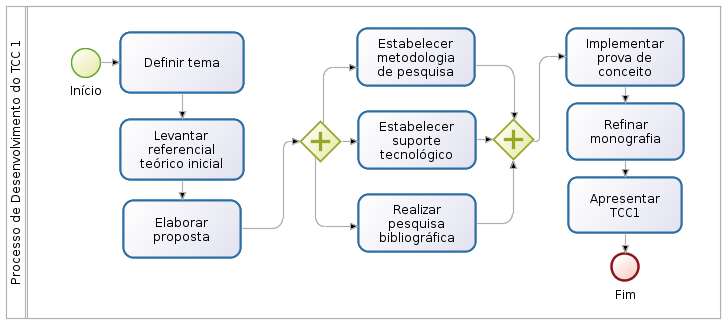
\includegraphics[scale=0.6]{figuras/processo_tcc1}
\caption{Processo de desenvolvimento do TCC1.}
\label{fig:proc_tcc1}
\end{figure}

As atividades descritas no processo de desenvolvimento do TCC1 (Figura \ref{fig:proc_tcc1}) são descritas brevemente a seguir:

\begin{itemize}
    \item \textbf{Definir tema:} envolve a identificação da área de pesquisa, discussão sobre possíveis temas de relevância.
    \item \textbf{Levantar referencial teórico inicial:} o referencial teórico que fundamenta a proposta e consolida o tema é levantado nesta atividade;
    \item \textbf{Elaborar proposta:} fomentar a pesquisa de modo a estabelecer seu escopo, objetivos, justificativa, questões de pesquisa, metodologia e cronograma de atividades mais elementares. Tais aspectos podem sofrer modificações ao decorrer do trabalho;
    \item \textbf{Estabelecer metodologia de pesquisa:} com maior familiaridade do pesquisador sobre o tema, a metodologia de pesquisa pode ser consolidada e classificada;
    \item \textbf{Estabelecer suporte tecnológico:} trata-se da indicação das ferramentas a serem utilizadas, as quais apoiaram em termos metodológicos o tema em investigação.
    \item \textbf{Realizar pesquisa bibliográfica:} envolve a pesquisa de trabalhos científicos que forneçam embasamento para os objetivos pré-estabelecidos;
    \item \textbf{Implementar prova de conceito:} implementação de prova de conceito para que sejam  identificados riscos potenciais que possam interferir na catalogação dos padrões;
    \item \textbf{Refinar monografia:} é averiguado se os objetivos do TCC1 foram atingidos bem como é refinada a escrita do mesmo;
    \item \textbf{Apresentar TCC1}: consiste na apresentação do TCC1 à banca examinadora.
\end{itemize}



\begin{figure}[!htb]
\centering
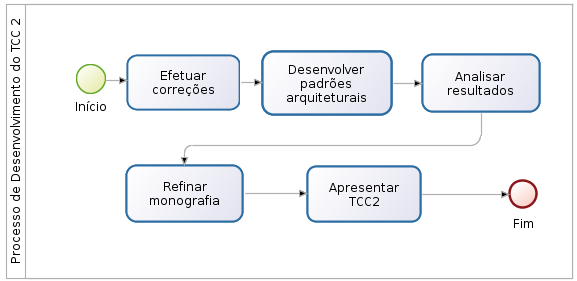
\includegraphics[scale=0.6]{figuras/processo_tcc2}
\caption{Processo de desenvolvimento do TCC2.}
\label{fig:proc_tcc2}
\end{figure}

\pagebreak

As atividades descritas no processo de desenvolvimento do TCC2 (Figura \ref{fig:proc_tcc2}) são descritas brevemente a seguir:

\begin{itemize}
    \item \textbf{Efetuar correções:} adequação da monografia às sugestões e críticas da banca examinadora.
    \item \textbf{Desenvolver padrões arquiteturais:} trata-se da implementação, modelagem e posterior catalogação dos padrões arquiteturais selecionado.
    \item \textbf{Analisar resultados:} (a fazer)
    \item \textbf{Refinar monografia:} é averiguado se os objetivos do TCC como um todo foram atingidos bem como é refinada a escrita do mesmo;
    \item \textbf{Apresentar TCC2:} apresentação do TCC2 à banca examinadora.
\end{itemize}

\section{Revisão sistemática}

(a fazer: o que é rs, pq vou usar rs)


Uma revisão sistemática da literatura, também referida como revisão sistemática, é um meio de identificar, avaliar e interpretar todas as pesquisas disponíveis relevantes para um determinado foco \cite{kitchenham2004}. 

Estudos individuais que contribuem com uma revisão sistemática são chamados estudos primários; uma revisão sistemática é uma forma de estudo secundário \cite{kitchenham2004}.

Dentre as razões para realizar uma revisão sistemática da literatura, destacam-se \cite{kitchenham2004}:
• Resumir a evidência existente sobre um tratamento ou tecnologia;
• Identificar eventuais lacunas na pesquisa atual, a fim de sugerir novas áreas de investigação;
• Fornecer um framework ou background, a fim de posicionar adequadamente novas atividades de investigação.

Em contraste com o processo habitual de revisão da literatura, não sistematicamente realizada sempre que um inicia um inquérito particular, um SR é desenvolvido, como o termo indica, de uma maneira formal e sistemática. Isto significa que o processo de condução de pesquisa de um tipo de avaliação sistemática segue uma sequência muito bem definida e rigorosa de passos metodológicos, de acordo com um protocolo desenvolvido aprioristicamente.


\subsection{Processo de revisão sistemática}

sampaio2007

\begin{figure}[!htb]
    \centering
    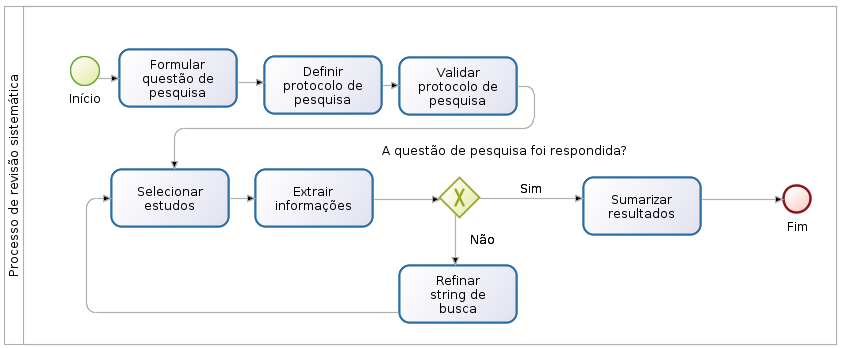
\includegraphics[scale=0.5]{figuras/processo_rs}
    \caption{Processo de revisão sistemática.}
    \label{fig:processo_rs}     
\end{figure}

\pagebreak


\subsection{Aplicação da revisão sistemática}

Foi elaborado o protocolo de revisão sistemática definido no Apêndice \ref{appendix:protocolo}. O objetivo é disponibilizar os procedimentos e decisões do processo de RS realizado de modo que possa ser repetido por outros pesquisadores que obterão os mesmos resultados. A estrutura deste protocolo baseou-se no trabalho de \citeonline{ramaiane2014}.


\section{Metodologia de desenvolvimento} \label{sec:metodologia_desenvolvimento}

Será adotada uma adaptação da metodologia Scrum para a atividade \textit{"Desenvolver padrões arquiteturais"} descrita na Figura \ref{fig:proc_tcc2}. 

\subsection{Scrum} \label{sec:scrum}

O Scrum é um \textit{framework} no qual pode-se resolver problemas complexos de forma produtiva com o principal objetivo de gerar produtos de maior valor possível \cite{schwaber2016}. Isto é favorecido empregando-se uma abordagem iterativa e incremental que promove controle de riscos e uma melhor previsão dos mesmos. O Scrum fundamenta-se no empirismo, afirmando que o conhecimento é desenvolvido pela experiência. São três os pilares que sustentam a implementação do processo empírico:

\par (i) transparência: aspectos significantes do processo devem ser visíveis para os responsáveis pelos resultados. A comunicação deve ser frequente e, consequentemente, estabelece confiança dos envolvidos;
\par (ii) inspeção: a transparência torna a inspeção possível. Envolve examinação atenciosa e \textit{feedbacks} constantes para tomar decisões com relação a adaptações no processo ou produto;
\par (iii) adaptação: a inspeção torna a adaptação possível. Adaptação diz respeito aos ajustes no produto em desenvolvimento ou no processo; o qual está sendo desenvolvido de acordo com os resultados da inspeção \cite{rubin2012}.

O objetivo da Scrum é entregar software de qualidade, tanto quanto possível, em intervalos curtos e fixos de tempo intitulados \textit{Sprints} \cite{beedle1999}. Cada fase do ciclo de desenvolvimento de software - consideradas por \citeauthor{beedle1999} (\citeyear{beedle1999}) como requisitos, análise, projeto, evolução e entrega) - é mapeada para uma \textit{Sprint} ou conjunto de \textit{Sprints} \cite{beedle1999}. Além da \textit{Sprint}, existem outros eventos prescritos no Scrum: \textit{Sprint Planning, Daily Scrum, Sprint Review, Sprint Retrospective}. Estes eventos são usados para criar regularidade de encontros do time bem como minimizar a necessidade de reuniões não definidas no Scrum. Cada um desses eventos requer que seja estabelecida uma duração máxima \cite{beedle1999}.

Para definir se o que foi produzido é potencialmente entregável, o time Scrum deve ter a definição de pronto - \textit{Definition of Done} (DoD)- bem estabelecida. A definição de pronto é um \textit{checklist} de tipos de trabalho que o time deve realizar completamente para declarar o trabalho desenvolvido na \textit{Sprint} como pronto \cite{rubin2012}.

Cada \textit{Sprint} opera com um certo número de itens de trabalho constituindo o \textit{Backlog}. Os papéis responsáveis pelo processo representam o \textit{Scrum Team}. Este é constituído por: \textit{Product Owner}, \textit{Development Team}, e um \textit{Scrum Master} \cite{beedle1999}.




\subsection{Processo de desenvolvimento}

Foram realizadas adaptações no \textit{Scrum} devido ao fato de haver somente um membro na equipe para compor o \textit{Scrum Team}. Portanto, serão utilizados: entregas a cada \textit{Sprint}, cerimônia \textit{Sprint Planning} e a utilização do \textit{Definition of Done}.
Serão adotados os procedimentos descritos na Figura \ref{fig:proc_desenv}. As \textit{Sprints} terão duração de duas semanas de modo que as histórias de usuário serão dadas como prontas seguindo a definição de pronto - ou \textit{Definition of Done} (ou "DoD"). 

\begin{figure}[!htb]
    \centering
    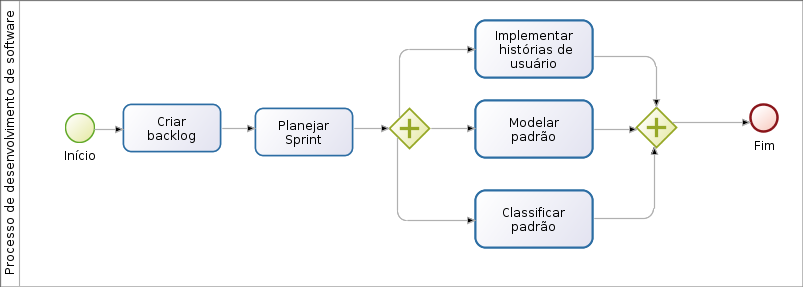
\includegraphics[scale=0.5]{figuras/processo_desenvolvimento.png}
    \caption{Processo de desenvolvimento de software.} 
    \label{fig:proc_desenv}
\end{figure}


\section{Metodologia de análise dos resultados}

(a fazer)

\section{Cronograma}

Os cronogramas referentes aos TCC 1 e 2 são definidos nas Tabelas \ref{tab:cronograma_1} e \ref{tab:cronograma_2}.

% ######## init table ########
\begin{table}[h]
 \centering \tiny 
 
% distancia entre a linha e o texto
 {\renewcommand\arraystretch{1.25}
 \caption{Cronograma de atividades do TCC1.}
 \label{tab:cronograma_1}
 \begin{tabular}{ l l l l l l }
  \cline{1-1}\cline{2-2}\cline{3-3}\cline{4-4}\cline{5-5}\cline{6-6}  
    \multicolumn{1}{p{4.750cm}|}{\textbf{Atividades} \centering } &
    \multicolumn{1}{p{1.383cm}|}{\textbf{Agosto} \centering } &
    \multicolumn{1}{p{1.383cm}|}{\textbf{Setembro} \centering } &
    \multicolumn{1}{p{1.400cm}|}{\textbf{Outubro} \centering } &
    \multicolumn{1}{p{1.417cm}|}{\textbf{Novembro} \centering } &
    \multicolumn{1}{p{1.400cm}}{\textbf{Dezembro} \centering }
  \\  
  \cline{1-1}\cline{2-2}\cline{3-3}\cline{4-4}\cline{5-5}\cline{6-6}  
    \multicolumn{1}{p{4.750cm}|}{Definir tema \centering } &
    \multicolumn{1}{p{1.383cm}|}{X \centering } &
    \multicolumn{1}{p{1.383cm}|}{  \centering } &
    \multicolumn{1}{p{1.400cm}|}{  \centering } &
    \multicolumn{1}{p{1.417cm}|}{  \centering } &
    \multicolumn{1}{p{1.400cm}}{  \centering }
  \\  
  %\cline{1-1}\cline{2-2}\cline{3-3}\cline{4-4}\cline{5-5}\cline{6-6}  
    \multicolumn{1}{p{4.750cm}|}{Levantar referencial teórico inicial \centering } &
    \multicolumn{1}{p{1.383cm}|}{X \centering } &
    \multicolumn{1}{p{1.383cm}|}{  \centering } &
    \multicolumn{1}{p{1.400cm}|}{  \centering } &
    \multicolumn{1}{p{1.417cm}|}{  \centering } &
    \multicolumn{1}{p{1.400cm}}{  \centering }
  \\  
  %\cline{1-1}\cline{2-2}\cline{3-3}\cline{4-4}\cline{5-5}\cline{6-6}  
    \multicolumn{1}{p{4.750cm}|}{Elaborar proposta \centering } &
    \multicolumn{1}{p{1.383cm}|}{X \centering } &
    \multicolumn{1}{p{1.383cm}|}{  \centering } &
    \multicolumn{1}{p{1.400cm}|}{  \centering } &
    \multicolumn{1}{p{1.417cm}|}{  \centering } &
    \multicolumn{1}{p{1.400cm}}{  \centering }
  \\  
  %\cline{1-1}\cline{2-2}\cline{3-3}\cline{4-4}\cline{5-5}\cline{6-6}  
    \multicolumn{1}{p{4.750cm}|}{Estabelecer metodologia de pesquisa \centering } &
    \multicolumn{1}{p{1.383cm}|}{  \centering } &
    \multicolumn{1}{p{1.383cm}|}{X \centering } &
    \multicolumn{1}{p{1.400cm}|}{  \centering } &
    \multicolumn{1}{p{1.417cm}|}{  \centering } &
    \multicolumn{1}{p{1.400cm}}{  \centering }
  \\  
  %\cline{1-1}\cline{2-2}\cline{3-3}\cline{4-4}\cline{5-5}\cline{6-6}  
    \multicolumn{1}{p{4.750cm}|}{Estabelecer suporte tecnológico \centering } &
    \multicolumn{1}{p{1.383cm}|}{  \centering } &
    \multicolumn{1}{p{1.383cm}|}{X \centering } &
    \multicolumn{1}{p{1.400cm}|}{  \centering } &
    \multicolumn{1}{p{1.417cm}|}{  \centering } &
    \multicolumn{1}{p{1.400cm}}{  \centering }
  \\  
  %\cline{1-1}\cline{2-2}\cline{3-3}\cline{4-4}\cline{5-5}\cline{6-6}  
    \multicolumn{1}{p{4.750cm}|}{Realizar pesquisa bibliográfica \centering } &
    \multicolumn{1}{p{1.383cm}|}{  \centering } &
    \multicolumn{1}{p{1.383cm}|}{X \centering } &
    \multicolumn{1}{p{1.400cm}|}{X \centering } &
    \multicolumn{1}{p{1.417cm}|}{  \centering } &
    \multicolumn{1}{p{1.400cm}}{  \centering }
  \\  
  %\cline{1-1}\cline{2-2}\cline{3-3}\cline{4-4}\cline{5-5}\cline{6-6}  
    \multicolumn{1}{p{4.750cm}|}{Implementar prova de conceito \centering } &
    \multicolumn{1}{p{1.383cm}|}{  \centering } &
    \multicolumn{1}{p{1.383cm}|}{  \centering } &
    \multicolumn{1}{p{1.400cm}|}{X \centering } &
    \multicolumn{1}{p{1.417cm}|}{X \centering } &
    \multicolumn{1}{p{1.400cm}}{  \centering }
  \\  
  %\cline{1-1}\cline{2-2}\cline{3-3}\cline{4-4}\cline{5-5}\cline{6-6}  
    \multicolumn{1}{p{4.750cm}|}{Refinar monografia \centering } &
    \multicolumn{1}{p{1.383cm}|}{  \centering } &
    \multicolumn{1}{p{1.383cm}|}{  \centering } &
    \multicolumn{1}{p{1.400cm}|}{  \centering } &
    \multicolumn{1}{p{1.417cm}|}{X \centering } &
    \multicolumn{1}{p{1.400cm}}{  \centering }
  \\  
  %\cline{1-1}\cline{2-2}\cline{3-3}\cline{4-4}\cline{5-5}\cline{6-6}  
    \multicolumn{1}{p{4.750cm}|}{Apresentar TCC1 \centering } &
    \multicolumn{1}{p{1.383cm}|}{  \centering } &
    \multicolumn{1}{p{1.383cm}|}{  \centering } &
    \multicolumn{1}{p{1.400cm}|}{  \centering } &
    \multicolumn{1}{p{1.417cm}|}{  \centering } &
    \multicolumn{1}{p{1.400cm}}{X \centering }
  \\  
  \hline

 \end{tabular} }
\end{table}

% ######## init table ########
\begin{table}[h]
 \centering \tiny
% distancia entre a linha e o texto
 {\renewcommand\arraystretch{1.25}
 \caption{Cronograma de atividades do TCC2.}
 \label{tab:cronograma_2}
 \begin{tabular}{ l l l l l l }
  \cline{1-1}\cline{2-2}\cline{3-3}\cline{4-4}\cline{5-5}\cline{6-6}  
    \multicolumn{1}{p{4.750cm}|}{\textbf{Atividades} \centering } &
    \multicolumn{1}{p{1.383cm}|}{\textbf{Fevereiro} \centering } &
    \multicolumn{1}{p{1.383cm}|}{\textbf{Março} \centering } &
    \multicolumn{1}{p{1.400cm}|}{\textbf{Abril} \centering } &
    \multicolumn{1}{p{1.417cm}|}{\textbf{Maio} \centering } &
    \multicolumn{1}{p{1.400cm}}{\textbf{Junho} \centering }
  \\  
  \cline{1-1}\cline{2-2}\cline{3-3}\cline{4-4}\cline{5-5}\cline{6-6}  
    \multicolumn{1}{p{4.750cm}|}{Efetuar correções \centering } &
    \multicolumn{1}{p{1.383cm}|}{X \centering } &
    \multicolumn{1}{p{1.383cm}|}{  \centering } &
    \multicolumn{1}{p{1.400cm}|}{  \centering } &
    \multicolumn{1}{p{1.417cm}|}{  \centering } &
    \multicolumn{1}{p{1.400cm}}{  \centering }
  \\  
  %\cline{1-1}\cline{2-2}\cline{3-3}\cline{4-4}\cline{5-5}\cline{6-6}  
    \multicolumn{1}{p{4.750cm}|}{Desenvolver padrões arquiteturais \centering } &
    \multicolumn{1}{p{1.383cm}|}{  \centering } &
    \multicolumn{1}{p{1.383cm}|}{X \centering } &
    \multicolumn{1}{p{1.400cm}|}{X \centering } &
    \multicolumn{1}{p{1.417cm}|}{X \centering } &
    \multicolumn{1}{p{1.400cm}}{  \centering }
  \\  
  %\cline{1-1}\cline{2-2}\cline{3-3}\cline{4-4}\cline{5-5}\cline{6-6}  
    \multicolumn{1}{p{4.750cm}|}{Analisar resultados \centering } &
    \multicolumn{1}{p{1.383cm}|}{  \centering } &
    \multicolumn{1}{p{1.383cm}|}{X \centering } &
    \multicolumn{1}{p{1.400cm}|}{X \centering } &
    \multicolumn{1}{p{1.417cm}|}{X \centering } &
    \multicolumn{1}{p{1.400cm}}{  \centering }
  \\  
  %\cline{1-1}\cline{2-2}\cline{3-3}\cline{4-4}\cline{5-5}\cline{6-6}  
    \multicolumn{1}{p{4.750cm}|}{Refinar monografia \centering } &
    \multicolumn{1}{p{1.383cm}|}{  \centering } &
    \multicolumn{1}{p{1.383cm}|}{  \centering } &
    \multicolumn{1}{p{1.400cm}|}{  \centering } &
    \multicolumn{1}{p{1.417cm}|}{X \centering } &
    \multicolumn{1}{p{1.400cm}}{X \centering }
  \\  
  %\cline{1-1}\cline{2-2}\cline{3-3}\cline{4-4}\cline{5-5}\cline{6-6}  
    \multicolumn{1}{p{4.750cm}|}{Apresentar TCC2 \centering } &
    \multicolumn{1}{p{1.383cm}|}{  \centering } &
    \multicolumn{1}{p{1.383cm}|}{  \centering } &
    \multicolumn{1}{p{1.400cm}|}{  \centering } &
    \multicolumn{1}{p{1.417cm}|}{  \centering } &
    \multicolumn{1}{p{1.400cm}}{X \centering }
  \\
  \hline

 \end{tabular} }
\end{table}





